\documentclass[a4paper,10pt]{report}
\usepackage[francais]{babel}
\usepackage{ucs}
\usepackage[utf8x]{inputenc}
\usepackage[T1]{fontenc}
\usepackage[pdftex]{graphicx}
\usepackage{xcolor}
\usepackage{textcomp}
\usepackage[top=2cm, bottom=2cm, left=1.5cm, right=1.5cm]{geometry}
\usepackage{amsmath} 
\usepackage{amssymb}
\usepackage{mathrsfs}
\usepackage{graphicx}
\usepackage{pgfgantt}

\usepackage{listings}
\definecolor{colKeys}{rgb}{0,0,1}
\definecolor{colIdentifier}{rgb}{0,0,0}
\definecolor{-}{rgb}{0,0.5,1}
\definecolor{colString}{rgb}{0.6,0.1,0.1}
\definecolor{colBack}{rgb}{0.9,0.9,0.9}
\definecolor{colComments}{rgb}{0.5,0.5,0.5}
\definecolor{mygreen}{RGB}{28,172,0} % color values Red, Green, Blue
\definecolor{mylilas}{RGB}{170,55,241}


\lstdefinestyle{customc}
{
  belowcaptionskip=1\baselineskip,
  breaklines=true,
  frame=L,
  xleftmargin=\parindent,
  language=C,
  numbers=left,
  showstringspaces=false,
  basicstyle=\footnotesize\ttfamily,
  keywordstyle=\bfseries\color{green!40!black},
  commentstyle=\itshape\color{purple!40!black},
  identifierstyle=\color{blue},
  stringstyle=\color{orange},
  tabsize=4,
}

\lstdefinestyle{customasm}
{
  belowcaptionskip=1\baselineskip,
  frame=L,
  xleftmargin=\parindent,
  language=[x86masm]Assembler,
  basicstyle=\footnotesize\ttfamily,
  commentstyle=\itshape\color{purple!40!black},
}

\lstset{language=Matlab,%
    %basicstyle=\color{red},
    breaklines=true,%
    morekeywords={matlab2tikz},
    keywordstyle=\color{blue},%
    morekeywords=[2]{1}, keywordstyle=[2]{\color{black}},
    identifierstyle=\color{black},%
    stringstyle=\color{mylilas},
    commentstyle=\color{mygreen},%
    showstringspaces=false,%without this there will be a symbol in the places where there is a space
    numbers=left,%
    numberstyle={\tiny \color{black}},% size of the numbers
    numbersep=9pt, % this defines how far the numbers are from the text
    emph=[1]{for,end,break},emphstyle=[1]\color{red}, %some words to emphasise
    %emph=[2]{word1,word2}, emphstyle=[2]{style},    
}

\lstset{escapechar=@,style=customc}

% Title Page
\title{Rapport MT44\\\huge{TP1}}
\author{Nicolas Fleurot\\Tony Duong}

\begin{document}
\maketitle

\tableofcontents

\chapter*{Introduction}
\addcontentsline{toc}{chapter}{Introduction}

    En mathématiques, en analyse numérique, l'interpolation polynomiale est une technique d'interpolation d'un ensemble de données ou d'une fonction par un polynôme. En d'autres termes, étant donné un ensemble de points $\lbrace{(t_{0}, y_{0}), … , (t_{n},y_{n})}\rbrace $ (obtenu, par exemple, à la suite d'une expérience, de mesures), on cherche un polynôme p de degré au plus n qui passe par tous ces points (donc tel que $p(t_{i}) = y_{i}$). 
\newline
\newline
    Dans une première partie, nous allons évaluer une fonction polynôme en $t$ avec ($t$ appartient réel) a partir d’un ensemble de points de support quelconque. Deux algorithmes seront utilisés afin d’évaluer cette fonction et nous comparerons les temps d’exécution respectifs. 
\newline
\newline
Dans une seconde partie, nous allons générer la table des différences divisés a partir des points de supports ainsi que l’écriture du polynôme d’interpolation en ayant calculé au préalable ses composantes. Nous mettrons ensuite en application ces outils MATLAB en utilisant des points régulièrement répartis ainsi que les huit points de Tchebyschev comme support pour notre polynôme d’interpolation de la fonction exponentielle.
\newline
\newline
Enfin, en utilisant les outils précédemment développés, nous mettrons en évidence l’erreur d’interpolation commise lors de l’approximation de la fonction exponentielle par les deux différentes fonctions d’interpolations (support avec répartition régulière et support de Tchebyschev).

\chapter*{Partie 1 : Evaluation d’une fonction polynôme en $t$}
\addcontentsline{toc}{chapter}{Partie 1 : Evaluation d’une fonction polynôme en $t$}

On considère la fonction polynôme $p$ de degré $n$ $(n \in N^{∗} )$ définie pour tout $x$
réel par son écriture de Newton relative aux centres $(c_{1} , ..., c_{n})$ :


\begin{equation}
p(x) = \sum_{\substack{i=0}}^{n} a_{i} \left(\prod_{j=1}^{i}(x-c_{i})\right)
\end{equation}

en adoptant les conventions du cours, c’est-à-dire :
\begin{list}{}{}
\item \begin{list}{$\bullet$}{}
\item $\prod^{0}_{j=1} (x-c_{j}) = 1$
\item les $a_{i}$ sont les composantes d’un vecteur de $n + 1$ réels définis plus haut,
\item $c$ désignera ci-dessous le vecteur des centres.
\end{list}
\end{list}

\section*{Question 1a}
\addcontentsline{toc}{section}{Question 1a}

\subsection*{Rappel}
\addcontentsline{toc}{subsection}{Rappel}

Ecrire une fonction d’évaluation de p en le réel t, notée $evaluation1(n, a, c, t)$, utilisant une fonction à définir, qui calcule les différents $\prod_{j=1}^{i}(x-c_{i})$
grâce à un schéma itératif. $evaluation1()$ fait usage des champs indiqués, conformément aux notations du poly, et produit $val = p(t)$.

\subsection*{Théorie}
\addcontentsline{toc}{subsection}{Théorie}

L’écriture du polynôme d’interpolation de Newton est la suivante :

\begin{equation}
p(x) = \sum_{\substack{i=0}}^{n} \left(a_{i}\left[\prod_{j=0}^{i-1}(x-x_{j})\right]\right)
\end{equation}

avec
\begin{itemize}
	\item[$a_{i}$] : les coefficients de newton
	\item[$x$]  : la valeur en laquelle la fonction sera évaluée
    \item[$x_{j}$] : les points de support
\end{itemize}
    
Pour calculer $p(t)$ avec $t$ un réel, nous devons d’abord calculer les différents $(t-c_{j})$ que nous conserverons dans un vecteur. Puis nous effectuons le produit des coefficients de l’écriture de Newton (qui sont considérés calculés avant l’appel de la fonction) par les différents polynômes de Newton stockés dans le vecteur.

\subsection*{Source}
\addcontentsline{toc}{subsection}{Source}

\begin{center}
	\lstinputlisting[caption=evaluation1, language=Matlab]{evaluation1.m}
\end{center}

\begin{center}
	\lstinputlisting[caption=product, language=Matlab]{Product.m}
\end{center}

\subsection*{Test}
\addcontentsline{toc}{subsection}{Test}

\begin{center}
	\lstinputlisting[caption=Test evaluation1, language=Matlab]{testevaluation1.m}
\end{center}

\section*{Question 1b}
\addcontentsline{toc}{section}{Question 1b}

\subsection*{Rappel}
\addcontentsline{toc}{subsection}{Rappel}

Dans cette partie, nous avons le même objectif que celui de la question précédente, à savoir calculer p(t) avec t un réel. Néanmoins nous devons utiliser non plus le schéma itératif mais le schéma de Horner. 

\subsection*{Théorie}
\addcontentsline{toc}{subsection}{Théorie}

Ecrire une fonction d’évaluation de $p$ en $t$, notée $evaluation(n, a, c, t →
val, nouv_a, nouv_c)$ qui utilise un schéma de Hörner et produit, en plus de
$val = p(t)$, le vecteur $nouv{a}$ des composantes de $p$ en écriture de Newton
relative à $nouv_c$ qui représente $(t, c_{1}, ..., c_{n−1})$ ainsi que le nouveau vecteur des centres.

\subsubsection*{Algorithme de Horner}

\textbf{entrée :}

\begin{list}{}{}
\item $n$ : entier naturel représentant le degré de $p$;
\item $a$ : vecteur de $n+1$ réels désignant les coefficients de $p$ dans la base considérée, donc $a(i) = a_{i}$ pour tout $i$ de $\lbrace 0, ..., n\rbrace$;
\item $c$ : vecteur de $n$ réels désignant les centres considérés, donc $c(i)=c_{i}$ pour tout $i$ de $\lbrace 1, ..., n\rbrace$;
\item $t$ : réel en lequel on évalue $p$;
\end{list}

\textbf{sortie}
\begin{list}{}{}
\item $val$ : réel défini par $val = p(t)$;
\item $a'$ : vecteur de $n+1$ réels, dont la signification profonde et l'utilité seront saisie dans le théorème 1.9;
\end{list}

\textbf{Début du corps}
\begin{list}{}{}
\item $a'(n) \longleftarrow a(n)$
\item \textbf{pour} i = n-1 à \textbf{faire}
\item \begin{list}{}{}
\item $a'(i) \longleftarrow a(i) + (t-c(i+1))a'(i+1)$
\end{list}
\item \textbf{fin pour}
\item $val \longleftarrow a'(0)$
\end{list}

\textbf{Fin du corps}

Nous étudierons ultérieurement la différence de performance entre ces deux schémas. 

\newpage
\subsection*{Source}
\addcontentsline{toc}{subsection}{Source}

\lstinputlisting[caption=product, language=Matlab]{evaluation.m}

\subsection*{Test}
\addcontentsline{toc}{subsection}{Test}

\begin{center}
	\lstinputlisting[caption=Test evaluation, language=Matlab]{testevaluation.m}
\end{center}

\section*{Question 1c}
\addcontentsline{toc}{section}{Question 1c}

\subsection*{Théorie}
\addcontentsline{toc}{subsection}{Théorie}

En utilisant les outils de Matlab $(tic, toc, etime, etc...)$ comparer les temps
d’exécution des deux fonctions d’évaluation écrites, en fonction du degré
du polynôme considéré. Visualiser les résultats obtenus.

\subsection*{Rappel}
\addcontentsline{toc}{subsection}{Rappel}

La performance est souvent très importante dans le calcul scientifique. C’est pourquoi nous comparons les temps d’exécution des deux algorithmes précédents en utilisant les fonctions tic et toc de Matlab.

\subsection*{Source / Test}
\addcontentsline{toc}{subsection}{Source / Test}

\begin{center}
	\lstinputlisting[caption=ExecTime1, language=Matlab]{ExecTime1.m}
\end{center}

\section*{Question 1d}
\addcontentsline{toc}{section}{Question 1d}

\subsection*{Théorie}
\addcontentsline{toc}{subsection}{Théorie}

Ecrire une version matricielle de $evaluation()$, qui à partir d’un vecteur
colonne de réels $T$ produit le vecteur colonne des images $p(T)$. Cette nouvelle
version sera conservée sous le même nom et considérée comme algorithme
d’évaluation par défaut.

\subsection*{Source}
\addcontentsline{toc}{subsection}{Source}

\lstinputlisting[caption=product, language=Matlab]{evaluation2.m}

\subsection*{Test}
\addcontentsline{toc}{subsection}{Test}

\begin{center}
	\lstinputlisting[caption=Test evaluation2, language=Matlab]{testevaluation2.m}
\end{center}

\chapter*{Partie 2 : Table des différences divisées et polynômes d’interpolation}
\addcontentsline{toc}{chapter}{Partie 2 : Table des différences divisées et polynômes d’interpolation}

On utilisera évidemment les algorithmes fournis en cours. On considère une
fonction $f$, connue sur un support $\lbrace x_{0},...,x_{n}\rbrace$, par la donnée pour tout $i$ de $\lbrace 0,...,n \rbrace$, de $y_{i}$ = $f(x_{i})$.

\section*{Question 2a}
\addcontentsline{toc}{section}{Question 2a}

\subsection*{Rappel}
\addcontentsline{toc}{subsection}{Rappel}

Ecrire une fonction $table\_diff\_div(x, y)$ qui, à partir des deux colonnes $x = (x_{0},...,x_{n})$ et $y = (f(x_{0}),...,f(x_{n}))$ de même taille, construit et affiche la table des différences divisées de $f$ sur le support considéré.

\subsection*{Théorie}
\addcontentsline{toc}{subsection}{Théorie}

Les différents coefficients ai de l’écriture de Newton se déterminent de la manière suivante : $a_{i} = f[x_{0},...,x_{n}] = \frac{f[x_{1},..,x_{k}]-f[x_{0},..,x_{k-1}]}{(x_{k}-x_{0})}$.
De plus, pour 1 point de support (support $\lbrace x_{0} \rbrace$), $f[x_{0}] = f(x_{0})$.
Pour 2 points de support (support $\lbrace x_{0},x_{1} \rbrace$), $f[x_{0},x_{1}] = \frac{f(x_{1})-f(x_{0})}{(x_{1}-x_{0})}$.
Ainsi, nous pouvons construire la table qui contiendra tous les coefficients de l’écriture de Newton à partir d’un support quelconque, appelé table des différences divisées.

\newpage
\subsection*{Source}
\addcontentsline{toc}{subsection}{Source}

\begin{center}
	\lstinputlisting[caption=table\_diff\_div, language=Matlab]{table_diff_div.m}
\end{center}

\subsection*{Test}
\addcontentsline{toc}{subsection}{Test}

\begin{center}
	\lstinputlisting[caption=Test table\_diff\_div, language=Matlab]{testtable_diff_div.m}
\end{center}

\section*{Question 2b}
\addcontentsline{toc}{section}{Question 2b}

\subsection*{Rappel}
\addcontentsline{toc}{subsection}{Rappel}

Ecrire une fonction $interpol(n, x, y)$ qui, à partir de l’entier naturel non
nul n, et des données x et y définies ci-dessus construit le vecteur des
composantes du polynôme d’interpolation $p_{n}$ de $f$ sur le support $\lbrace  x_{0},...,x_{n} \rbrace$,
ainsi que la chaîne de son écriture.

\subsection*{Théorie}
\addcontentsline{toc}{subsection}{Théorie}

Les coefficients de Newton sont situés sur la diagonale descendante de la table des différences divisées. 

L’écriture de Newton est de la forme :

\begin{equation}
p(x) = \sum_{\substack{i=0}}^{n} \left(a_{i}\left[\prod_{j=0}^{i-1}(x-x_{j})\right]\right)
\end{equation}

Ainsi, nous utilisons la fonction précédente générant la table des différences divisés afin de récupérer les coefficients de l’écriture de Newton. Après cela, nous affichons sa chaîne de caractères pour mettre en évidence sa constitution. 

\newpage
\subsection*{Source}
\addcontentsline{toc}{subsection}{Source}

\begin{center}
	\lstinputlisting[caption=interpol, language=Matlab]{interpol.m}
\end{center}

\subsection*{Test}
\addcontentsline{toc}{subsection}{Test}

\begin{center}
	\lstinputlisting[caption=Test interpol, language=Matlab]{testinterpol.m}
\end{center}

\section*{Question 2c}
\addcontentsline{toc}{section}{Question 2c}

\subsection*{Rappel}
\addcontentsline{toc}{subsection}{Rappel}

\begin{list}{}{}
\item \begin{list}{$\bullet$}{}
\item Déterminer le polynôme d’interpolation $p_{7,1}$ de la fonction exp sur
le support $X1$ des huits points régulièrement répartis sur l’intervalle [1, 1].
\item Déterminer le polynôme d’interpolation $p_{7,2}$ de la fonction $exp$ sur le
support $X2$ des huits points de Tchebyschev, définis par : $\forall j \in \lbrace 0,...,7 \rbrace$  $X2_{j} = cos(\frac{2j+1}{8} \frac{\pi}{2}).$
\end{list}
\end{list}

\subsection*{Théorie}
\addcontentsline{toc}{subsection}{Théorie}

Nous mettons ici en application les outils précédemment développés pour interpoler la fonction exponentielle sur deux supports différents et pour afficher les écritures respectives.

Les supports sont :
\begin{list}{}{}
\item \begin{list}{$\bullet$}{}
\item le support des huit points régulièrement répartis sur l’intervalle [-1,1].
\item le support des huit points de Tchebyschev définis par : $\forall j \in \lbrace 0,...,7 \rbrace$  $X2_{j} = cos(\frac{2j+1}{8} \frac{\pi}{2}).$

\end{list}
\end{list}

\newpage
\subsection*{Source / Test}
\addcontentsline{toc}{subsection}{Source / Test}

\begin{center}
	\lstinputlisting[caption=ApplicationExp, language=Matlab]{ApplicationExp.m}
\end{center}

\begin{center}
	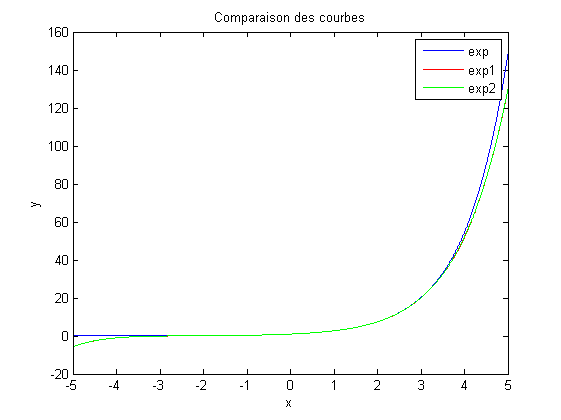
\includegraphics[scale=0.8]{comparaison.png}
\end{center}

Nous remarquons que plus on s'éloigne du domaine d'étude (ici, intervalle [-1;1]), plus la différence entre la courbe de la fonction exponentielle et celles des fonctions interpôlantes augmente. Ceci est cohérent.

\chapter*{Partie 3 : Visualisation de l’erreur d’interpolation}
\addcontentsline{toc}{chapter}{Partie 3 : Visualisation de l’erreur d’interpolation}

\subsection*{Rappel}
Utiliser la question précédente et les outils antérieurement développés, pour
visualiser sur une même représentation graphique, la valeur absolue de l’erreur
d’interpolation commise lors de l’approximation de la fonction exponentielle
par $p_{7,1}$ et $p_{7,2}$.


\subsection*{Théorie}
Nous utilisons ici les outils antérieurement développés pour calculer l'erreur entre la fonction exponentielle connu et son approximation par $p_{7,1}$ et $p_{7,2}$.
Nous utiliserons la formule
\begin{equation}
	e_{n}(t) = f(t) - p_{n}(t)
\end{equation}

avec

\begin{list}{}{}
\item
\begin{itemize}
	\item[$e_{n}(t)$]: Erreur de l'approximation.
	\item[$f(t)$]: Fonction exponentielle.
	\item[$p_{n}(t)$]: Approximation de la fonction exponentielle.
\end{itemize}
\end{list}

\subsection*{Source}
\addcontentsline{toc}{subsection}{Source}
\begin{center}
	\lstinputlisting[caption=Erreur, language=Matlab, mathescape]{ErreurTex.m}
\end{center}

\subsection*{Test}
\addcontentsline{toc}{subsection}{Test}

\begin{center}
	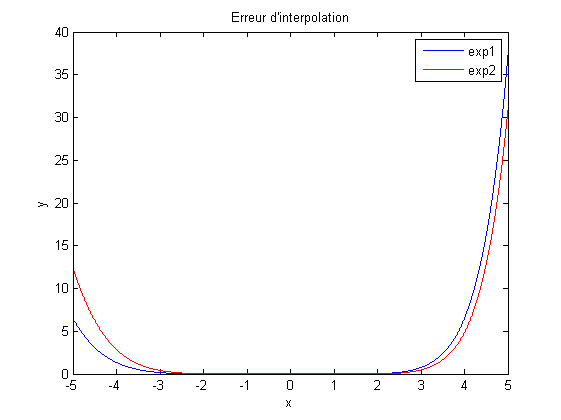
\includegraphics[scale=0.8]{erreur.png} 
\end{center}

\begin{center}
	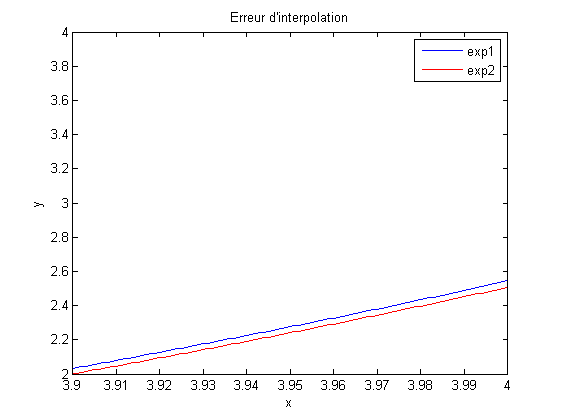
\includegraphics[scale=0.8]{zoomErreur2.png} 
\end{center}

Dès que l'on s'éloigne de l'intervalle [-1;1], l'erreur avec le support de Tchebyschev devient plus petite que l'erreur avec le support des points équidistants. C'est l'avantage d'utiliser ces points si on souhaite une fonction qui approxime correctement même en dehors de l'intervalle d'étude.

\chapter*{Conclusion}
\addcontentsline{toc}{chapter}{Conclusion}

La problématique de ce chapitre a été de pouvoir trouver une fonction polynôme qui passerait par un nombre fini de points d’un certain support (obtenus par mesures par exemples). Il existe plusieurs méthodes pour arriver à ce but.
\newline
\newline
Dans ce TP, nous avons utilisé la méthode de Newton et avons produit deux algorithmes permettant d’évaluer la fonction en un point quelconque t. La fonction supposait que l’on connaissait à l’avance les coefficients de l’écriture de Newton.
\newline
\newline
Le premier algorithme produit est classique : il consiste à calculer les polynômes $(x-c)$ où $c$ est un point du support et à multiplier ceux-ci par leurs coefficients respectifs. Néanmoins, cette méthode génère des répétitions et n’est donc pas optimal en terme de temps d’éxécution.
\newline
\newline 
La seconde méthode tiré du Schéma de Horner n’a pas ce défaut. En effet, étant donné que les facteurs $(x-c)$ sont répétés dans l’écriture, il était préférable d’ajouter les facteurs déjà calculés aux les termes suivants de la somme.
\newline
\newline
La mesure du temps d’exécution confirme notre affirmation.
\newline
\newline
Par la suite, nous nous sommes intéressés par l’écriture de la fonction interpôlante en générant la table des différences divisées (qui contient les coefficients de Newton) et en écrivant cette écriture sous forme de chaîne de caractères. Nous devions ensuite interpôler la fonction exponentielle. 
\newline
\newline
Mais la question la plus importante concerne l’erreur commise en faisant cette approximation et le choix des points de support. L’erreur aux points de support est bien sûr nulle mais qu’en est-il des autres points ? 
\newline
\newline


\end{document}